\chapter{Evaluation}
In this chapter, the workflow explained in last chapter is evaluated and results are
presented.

Before showing the evaluation, it is necessary to define training and testing conditions
that can be easily used by others to verify the results.

Each evaluation has a setup and its corresponding result.

We have three datasets that can be used for training and evaluation.
\begin{enumerate}
    \item Dataset 1 - Contains 100,000 raw data. It is collected in no traffic
        environment, doing straight driving without any sudden turning. The data is using
        San Francisco map and driven during afternoon. This dataset has only data
        representing centre camera pointed ahead, parallel to the ground and right camera
        pointed to the ground at an angle $20^{\circ}$. The control commands include
        acceleration, throttle, braking, and steering angle values.
    \item Dataset 2 - Also contains 100,000 raw data. It is, however, collect with traffic
        where the cars stop at signal intersections for a longer time than dataset 3. This
        dataset is also collect in San Francisco map and during afternoon. It contains a
        centre camera, right camera like dataset 1, left camera similar to right camera by
        pointing at an angle $20^{\circ}$ to the ground, depth camera sensors placed at
        centre, left and right just like RGB cameras. The control commands are same as
        dataset 1.
    \item Dataset 3 - Contains 270,000 raw data. It is collected while driving around San
        Francisco. About 200,000 data is collected while driving in the afternoon. About
        20,000 in different weather and light conditions. About 50,000 entries are
        collected in a different circular circuit map called CubeTown. In addition to RGB
        and depth cameras distributed just as dataset 2, a segmentation camera is kept
        next centre RGB camera facing forward, and a radar sensor just in front of the
        car near the hood also facing forward.

\end{enumerate}
\begin{figure}
    \centering
    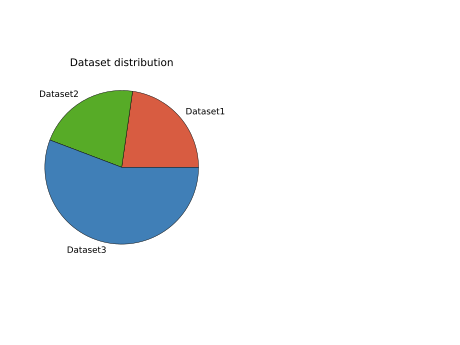
\includegraphics[width=0.5\textwidth]{figures/png/datasets_general.png}
    \caption{Datasets distribution}
    \label{fig:datasetsdistribution}
\end{figure}

\section{Evaluation setup}
While evaluating, a testing parameter \textit{episode} is used. Each episode lasts 30 seconds. A timer is started for 30 seconds and
the  model is tested for collisions. If a collision happens, the time at which collision
happened is noted.

\subsection{Setup 1 - Determine the best lighting conditions to test the model}
\label{chapter05subsec:setup1}
All three datasets are used. The test is conducted in San Franciso map without traffic
option switched ON. By varying the light conditions to morning, afternoon and evening, we
observe how light influences the prediction of output. Only steering angle is predicted
and a steady velocity of 3 meter per second is used. An episode length of 30s is used.
When a collision is observed, the time of collision and the count are noted down.
\begin{table}[t]
    \centering
\begin{tabular}{|c c c c|}
    \hline
    time(in 24 hrs standard) & Morning & Afternoon & Evening \\\hline
      & 7:35 & 15:30 & 18:30 \\\hline
\end{tabular}
\caption{Time of the day}
\label{table:timeoftheday}
\end{table}

\begin{figure}
	\centering
    \def\svgwidth{0.6\textwidth}
    \input{figures/inkscape/datasetsLCCollisions.pdf_tex} %use full path to know the location of pdftex
    \caption{Datasets vs Light Conditions vs Number of Collisions}
    \label{fig:dsvslcvsncolsetup1}
\end{figure}

It is seen from figure \ref{fig:dsvslcvsncolsetup1} that afternoon time provides the best light conditions for all the three
datasets. Dataset 1 and 3 perform equally across the three lighting conditions.

If the percentage of number of collisions, as shown in figure
\ref{fig:dsvslcvstrafficavgncolsetup1a}, is calculated, dataset 3 performs the best among
the datasets for morning and afternoon part of the day.
\begin{figure}
	\centering
    \def\svgwidth{0.6\textwidth}
    \input{figures/inkscape/averagecollisionsSetup1.pdf_tex} %use full path to know the location of pdftex
    \caption{Datasets vs Afternoon vs Traffic vs Average number of Collisions}
    \label{fig:dsvslcvstrafficavgncolsetup1a}
\end{figure}

\subsection{Setup 2 - How the datasets perform during afternoon if traffic is enabled?}
All three datasets are again used. The time is fixed at 15:30. The traffic is toggled ON.

\begin{figure}
	\centering
    \def\svgwidth{0.6\textwidth}
    \input{figures/inkscape/Afternoonwithtraffic.pdf_tex} %use full path to know the location of pdftex
    \caption{Datasets vs Afternoon vs Traffic vs Number of Collisions}
    \label{fig:dsvslcvstrafficncolsetup2}
\end{figure}
From figure \ref{fig:dsvslcvstrafficncolsetup2}, we can observe that all three datasets do
well even in traffic. However, it is surprising to see dataset 1 which had no traffic
while the dataset was collected, performs remarkably well when driven in traffic.
\subsection{LSTM vs Non-LSTM}
In the next stage of evaluation, acceleration in addition to steering is predicted.
Acceleration in LGSVL contains positive values for forward throttle and negative values
for braking.

Acceleration is relative to previous frame. Hence it is necessary to include past frames
information while predicted it. LSTM is used for this purpose. When non-LSTM model is used
to predict acceleration, it only predicts for the current frame which often results in
vehicle being stationary.

For our setup, we choose a $timestep = 15$. That means acceleration of current time frame
is predicted using previous 15 time frames.

\subsection{Regression models - Acceleration and Steering}
\subsubsection*{Determining the optimal LSTM output units}
In the table \ref{table:unitsvstime}, we can see that for 100 LSTM output units, though
the trainable parameters(parameters that can be trained during backpropagation) is quite compared to other units, the training time is the least.
Moreover on evaluation, it is observed that acceleration prediction is relatively good
compared to other units' models. Hence, a LSTM unit of 100 is chosen.
\begin{table}[t]
    \centering
\begin{tabular}{|c c c|}
    \hline
    LSTM Output Units & Trainable Parameters & Processing time needed \\\hline
    20 & 20000 & 1hr 44m  \\\hline
    60 & 61000 & 1hr 42m \\\hline
    100 & 434000  & 1hr 40m \\\hline
\end{tabular}
\caption{LSTM Output Units vs Training time}
\label{table:unitsvstime}
\end{table}
\begin{figure}[h]
	\centering
    \def\svgwidth{\textwidth}
    \input{figures/inkscape/regressionModelsTanhActivation.pdf_tex} %use full path to know the location of pdftex
    \caption{Datasets 1 vs 3 - Acceleration and Steering using Tanh activation and MSE loss
    functions.}
    \label{fig:ds1and3tanhactivatonMSE}
\end{figure}
\begin{figure}[h]
	\centering
    \def\svgwidth{\textwidth}
    \input{figures/inkscape/regressionModelsSigActivation.pdf_tex} %use full path to know the location of pdftex
    \caption{Datasets 1 vs 3 - Acceleration and Steering using Sigmoid activation and MSE loss
    functions.}
    \label{fig:ds1and3SigactivatonMSE}
\end{figure}
\begin{figure}[h]
	\centering
    \def\svgwidth{\textwidth}
    \input{figures/inkscape/regressionModelsSigActivationDS3.pdf_tex} %use full path to know the location of pdftex
    \caption{Dataset 3 - Acceleration and Steering using Sigmoid activation and MSE loss
    functions with adjusted dense layers.}
    \label{fig:ds3SigactivatonMSE}
\end{figure}

\subsection{Classification and Regression models}
\subsubsection*{Binary Crossentropy}
\begin{figure}[h]
	\centering
    \def\svgwidth{\textwidth}
    \input{figures/inkscape/BinaryCross2.pdf_tex} %use full path to know the location of pdftex
    \caption{Dataset 1 - Binary Crossentropy}
    \label{fig:ds1binarycrossentropy}
\end{figure}

\begin{figure}[h]
	\centering
    \def\svgwidth{\textwidth}
    \input{figures/inkscape/BinaryCross2ds3.pdf_tex} %use full path to know the location of pdftex
    \caption{Dataset 3 - Binary Crossentropy}
    \label{fig:ds3binarycrossentropy}
\end{figure}
\subsubsection*{Categorical Crossentropy - a basic model}
\begin{figure}[h]
	\centering
    \def\svgwidth{\textwidth}
    \input{figures/inkscape/categoricalcrossds1.pdf_tex} %use full path to know the location of pdftex
    \caption{Dataset 1 - Categorical Crossentropy}
    \label{fig:ds1categoricalcrossentropy}
\end{figure}

\begin{figure}[h]
	\centering
    \def\svgwidth{\textwidth}
    \input{figures/inkscape/categoricalcrossds3.pdf_tex} %use full path to know the location of pdftex
    \caption{Dataset 3 - Categorical Crossentropy}
    \label{fig:ds3categoricalcrossentropy}
\end{figure}
\begin{figure}[h]
    \centering
    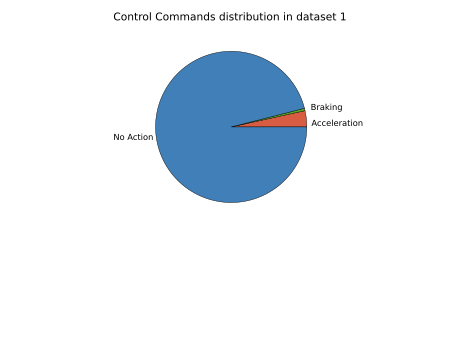
\includegraphics[width=0.5\textwidth]{figures/png/dataset1_control_cmds.png}
    \caption{Dataset 1 Control commands distribution}
    \label{fig:dataset1ctrlcmds}
\end{figure}
\begin{figure}[h]
    \centering
    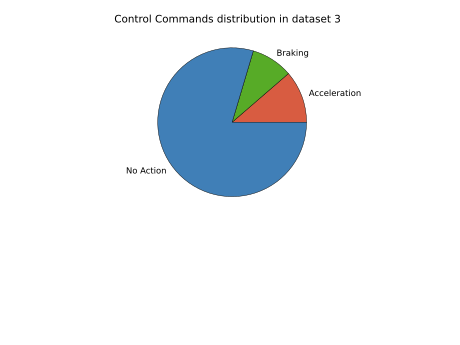
\includegraphics[width=0.5\textwidth]{figures/png/dataset3_control_cmds.png}
    \caption{Dataset 3 Control commands distribution}
    \label{fig:dataset3ctrlcmds}
\end{figure}

\subsubsection*{Categorical Crossentropy - splitting at the dense layers}
\begin{figure}[h]
	\centering
    \def\svgwidth{\textwidth}
    \input{figures/inkscape/categoricalcrossds3dense.pdf_tex} %use full path to know the location of pdftex
    \caption{Dataset 3 - Categorical Crossentropy - Separate dense layers for
    classification and steering}
    \label{fig:ds3categoricalcrossentropydense}
\end{figure}
\subsubsection*{Categorical Crossentropy - splitting at the LSTM layers}
\begin{figure}[h]
	\centering
    \def\svgwidth{\textwidth}
    \input{figures/inkscape/categoricalcrossds3lstm.pdf_tex} %use full path to know the location of pdftex
    \caption{Dataset 3 - Categorical Crossentropy - Separate LSTM layers for
    classification and steering}
    \label{fig:ds3categoricalcrossentropylstm}
\end{figure}
\subsubsection*{Categorical Crossentropy - Using two different NN for acceleration and
Steering}
\begin{figure}[h]
	\centering
    \def\svgwidth{\textwidth}
    \input{figures/inkscape/categoricalcrossds32nn.pdf_tex} %use full path to know the location of pdftex
    \caption{Dataset 3 - Categorical Crossentropy - Separate neural network for
    Classification and Steering}
    \label{fig:ds3categoricalcrossentropy2nn}
\end{figure}

\begin{figure}[h]
	\centering
    \def\svgwidth{\textwidth}
    \input{figures/inkscape/categoricalcrossds3steeringCompare.pdf_tex} %use full path to know the location of pdftex
    \caption{Dataset 3 - Categorical Crossentropy - Steering command loss comparison}
    \label{fig:ds3categoricalcrossentropysteeringcompare}
\end{figure}

\begin{figure}[h]
	\centering
    \def\svgwidth{0.5\textwidth}
    \input{figures/inkscape/steeringbasicmodel.pdf_tex} %use full path to know the location of pdftex
    \caption{Dataset 3 - Categorical Crossentropy - Basic model}
    \label{fig:steeringbasicmodel}
\end{figure}
\begin{figure}[h]
	\centering
    \def\svgwidth{0.5\textwidth}
    \input{figures/inkscape/steeringdensesplit.pdf_tex} %use full path to know the location of pdftex
    \caption{Dataset 3 - Categorical Crossentropy - Split at the second dense layer}
    \label{fig:steeringdensesplit}
\end{figure}
\begin{figure}[h]
	\centering
    \def\svgwidth{0.5\textwidth}
    \input{figures/inkscape/steeringlstmsplit.pdf_tex} %use full path to know the location of pdftex
    \caption{Dataset 3 - Categorical Crossentropy - Split at the LSTM layer}
    \label{fig:steeringlstmsplit}
\end{figure}
\begin{figure}[h]
	\centering
    \def\svgwidth{0.5\textwidth}
    \input{figures/inkscape/steeringNNsplit.pdf_tex} %use full path to know the location of pdftex
    \caption{Dataset 3 - Categorical Crossentropy - Separate NN training model}
    \label{fig:steeringnnsplit}
\end{figure}
\subsection{Velocity}






\begin{figure}
	\centering
    \def\svgwidth{\textwidth}
    \input{figures/inkscape/carsensors.pdf_tex} %use full path to know the location of pdftex
    \caption{Sensor Constellation}
    \label{fig:simplesensorconstellation}
\end{figure}

\iffalse
-----------------------------

\textbf{Dataset 1} - 100k raw data with no traffic. Just driving straight. First one with just steering and no other training.  With 1 centre camera.

\textbf{Dataset 2} - 100k raw data with traffic and increased wait times at junctions.

\textbf{Dataset 3} - 270K raw data with normal waiting times, increased brake scenario, different weather and light conditions, also driving in different map. With segmentation and radar.

----------------------------

\subsection{Test scenario 1}

----------------

\textbf{Epsiodes} - One minute. Manually start timer and run the evaluation. Count the \# of collisions. If collided, reset episode and start again. If no collision, restart after episode duration(1 min).


\subsection{Test Scenario 2}

---------------

Loss function as constant and using dataset 3. Explain why dataset 3 is being chosen.

CNN architecture should be same!

\textbf{MSE} - output(accel, brake and steering all regression)

\textbf{CCE} - input images(center and center depth). Output(Accel, brake and steering mse)

\textbf{With no traffic} -

Drive for 1 hour and see how model responds.

\textbf{With traffic} -

drive for 1 hour and see how model responds.

Epoch training - 50
\section{Testbed setup}

\begin{enumerate}
    \item dataset constant - Only dry day data?
        or everything?
    \item CNN parameters variable.
    \item epochs, learning rate, optimizer, loss function constant
    \item activation function constant or variable?
    \item for LSTM - timesteps value?
    \item graph - training, val loss vs epochs?
    \item graph - loss vs learning rate?
    \item graph - timesteps vs loss?
    \item graph - evaluation performance comparison?
    \item graph - Accel, brake, noaction predicted vs ?
    \item graph - brake, steering predicted vs ?
    \item graph - accel, brake, steering predicted vs ?
    \item graph - accel,brake, steering, distance(radar) predicted vs ?
    \item graph - with seg camera vs without?
    \item graph - with radar vs without?
    \item graph - imbalanced vs balanced Cross entropy?


\end{enumerate}
\fi
